%~~~~~~~~~~~~~~~~~~~~~~~~~~~~~~~~~~~~~~~~~~~~~~~~~~~~~~~~~~~~~~~~~~~~~~~
\section{\emph{MinHash}}\label{sec:minhash}
%~~~~~~~~~~~~~~~~~~~~~~~~~~~~~~~~~~~~~~~~~~~~~~~~~~~~~~~~~~~~~~~~~~~~~~~

\emph{MinHash} é um algoritmo \emph{hash}ing sensível a localização que permite estimar a semelhança entre conjuntos de forma indireta, através da aproximação do coeficiente de similaridade de \emph{Jaccard}. 

O algoritmo foi inventado por Andrei Broder \cite{broder1997resemblance} como forma de detectar páginas quase-duplicadas no mecanismo de busca Alta Vista. Antes disso, Heintze \cite{heintze1996scalable} e Manber \cite{manber1994finding} já haviam descrito um mecanismo de \emph{fingerprinting} de documentos para rápida indexação e busca por similaridade.  Entretanto, somente com o artigo de Broder, a técnica ganhou mais notoriedade.

\emph{MinHash} possui muitas aplicações. A principal envolve a detecção de documentos quase duplicados, através da representação dos mesmos como o conjunto de palavras ou n-gramas que contêm. O algoritmo, entretanto, possui aplicações diversas, desde sistemas de recomendação \cite{das2007google} até técnicas processamento de som \cite{chiu2010background,covell2007known}.

\subsection{Definição}

O objetivo do algoritmo \emph{MinHash} é estimar o coeficiente de Jaccard. Este coeficiente é definido, para dois conjuntos $A$ e $B$, como a razão entre a cardinalidade da interseção e a cardinalidade da união dos conjuntos \cite{real1996probabilistic}.
\[
J(A, B) = \frac{| A \cap B |}{| A \cup B|}
\]

O coeficiente $J(A, B)$ assume valores entre 0 e 1, sendo 0 para $A$ e $B$ disjuntos e 1 para $A$ e $B$ idênticos. Por exemplo, para os conjuntos:
\[
\begin{split}
A &= \{1, 3, 7, 14, 20\}\ \text{e} \\
B &= \{1, 3, 7, 19, 20, 35\}\text{,}
\end{split}
\]

o valor do coeficiente é:
\[
J(A, B) = \frac{ |\{1, 3, 7, 20 \}| }{ |\{1, 3, 7, 14, 19, 20, 35\}| } = \frac{4}{7} = 0.571428\dots
\]

Embora seja trivial calcular o coeficiente de \emph{Jaccard}, pode ser computacionalmente custoso realizar a comparação entre muitos pares de conjuntos com números muito grandes de elementos. Por isso, pode ser vantajoso pré-processar informações para cada conjunto que auxiliem na posterior aproximação do coeficiente. Em sua variante básica, tal pré-processamento consiste em aplicar um número constante de funções \emph{hash} sobre cada elemento de um conjunto e guardar o mínimo valor obtido para cada função. O resultado obtido é chamado de \emph{assinatura} do conjunto. Usando as assinaturas de cada conjunto é possível estimar a semelhança entre eles em tempo constante \cite{broder1997resemblance}, como veremos logo adiante.

A matriz característica é uma matriz binária $M$ na qual cada linha está mapeada a um elemento de $S_1 \cup S_2 \cup \cdots \cup S_n$ e a i-ésima coluna está mapeada a $S_i$. Cada posição na matriz é tal que $M[e, i] = 1$ se $e \in S_i$, para todo $e \in S_1 \cup S_2 \cup \cdots \cup S_n$. Considere, por exemplo, os conjuntos
\[
    S_1 = \{a, d\} \text{, } 
    S_2 = \{c\} \text{, } 
    S_3 = \{b, d, e\} \text{ e }
    S_4 = \{a, c, d\} \text{.}
\]

Portanto, $S_1 \cup S_2 \cup S_3 \cup S_4 = \{a, b, c, d, e\}$ e uma matriz característica associada é aquela da Figura~\ref{fig:minhash_charmatrix}.

\begin{figure}[!htbp]
\centering
\begin{tabular}{ c || c | c | c | c }
 elemento & $S_1$ & $S_2$ & $S_3$ & $S_4$ \\
\hline
  $a$ & 1   & 0   & 0   & 1   \\
  $b$ & 0   & 0   & 1   & 0   \\
  $c$ & 0   & 1   & 0   & 1   \\
  $d$ & 1   & 0   & 1   & 1   \\
  $e$ & 0   & 0   & 1   & 0   \\
\end{tabular}
\caption{Matriz característica para os conjuntos $S_1$, $S_2$, $S_3$ e $S_4$.}
\label{fig:minhash_charmatrix}
\end{figure}

Esta matriz característica geralmente não é a estrutura de dados usada na implementação dos conjuntos, e sim apenas uma forma conveniente de representá-los para facilitar a compreensão do algoritmo.

Para computar a assinatura de um conjunto, primeiro obtemos uma permutação das linhas da matriz característica anterior. Assim, a assinatura $h_{\min}(S)$ de um certo conjunto $S$ é definido pelo primeiro elemento na permutação que pertence a $S$.

Considere no exemplo a permutação $\{b, e, a, d, c\}$. A partir dela, podemos reorganizar a matriz característica como mostrado na Figura~\ref{fig:minhash_charmatrix_permutated}.

\begin{figure}[!htbp]
\centering
\begin{tabular}{ c || c | c | c | c }
 elemento & $S_1$ & $S_2$ & $S_3$ & $S_4$ \\
\hline
  $b$ & 0   & 0   & \colorbox{gray!30}{\textbf{1}}   & 0   \\
  $e$ & 0   & 0   & 1   & 0   \\
  $a$ & \colorbox{gray!30}{\textbf{1}}   & 0   & 0   & \colorbox{gray!30}{\textbf{1}}   \\
  $d$ & 1   & 0   & 1   & 1   \\
  $c$ & 0   & \colorbox{gray!30}{\textbf{1}}   & 0   & 1   \\
\hline

  \textbf{\emph{min hash}} & a & c & b & a \\

\end{tabular}
\caption{Matriz permutada, destacando o \emph{min hash} de cada conjunto.}
\label{fig:minhash_charmatrix_permutated}
\end{figure}


Broder \cite{broder1997resemblance} mostra que, para dois conjuntos $A$ e $B$, e um \emph{min hash} $h_{\min}$ aleatoriamente escolhidos, a probabilidade de terem o mesmo valor para $h_{\min}$ é igual ao próprio índice de \emph{Jaccard}, conforme se demonstra a seguir.

Parte-se do princípio que, considerando as colunas para os conjuntos $A$ e $B$ na matriz característica, os conjuntos $X$, $Y$ e $Z$ particionam o conjunto das linhas de $M$: onde ambas as colunas têm valor \textbf{1} (subconjunto $X$ de linhas), onde cada coluna tem um valor diferente (subconjunto $Y$ de linhas) e onde ambas as linhas têm valor \textbf{0} (subconjunto $Z$ de linhas).

Por um lado, $J(A, B) = |X|/(|X|+|Y|)$, pois $X$ representa $A \cap B$ e $Y$ representa $A \cup B - A \cap B$. Por outro lado, dada uma permutação aleatória da matriz, a probabilidade que uma linha em $X$ apareça antes de uma linha em $Y$ (i.e. $h_{\min}(A) = h_{\min}(B)$) antes de uma linha do tipo $Y$ (i.e. $h_{\min}(A) \neq h_{\min}(B)$) é exatamente $|X|/(|X|+|Y|)$. Portanto,
\[
\Pr[h_{\min}(A) = h_{\min}(B)] = J(A, B)
\]

É possível, assim, definir um estimador não-enviesado para o índice de \emph{Jaccard}
\[ 
   \hat{J}(A, B) = \mathds{1}(h_{\min}(A) = h_{\min}(B))
\]

onde
\[
\mathds{1}(b) = \begin{cases} 
    1 & \text{se}\ b = \textsc{Verdadeiro} \\
    0 & \text{se}\ b = \textsc{Falso} \\
\end{cases}
\]

Este estimador, entretanto, assume apenas os valores $0$ ou $1$ exatamente. Possui, portanto, uma grande variância em relação ao valor esperado. Entretanto, serve como ponto de partida para as duas principais variantes do algoritmo, como veremos a seguir.

\subsection{Exemplo}\label{sec:minhash:example}


\subsection{Variante com múltiplas funções \emph{hash}}

Uma variante simples do algoritmo \emph{MinHash} utiliza múltiplas funções \emph{hash} para gerar vários estimadores e, através da média simples entre eles, estimar o índice de \emph{Jaccard}. 

Isto é, utiliza-se $k$ funções \emph{hash} $\{h_1, h_2, ... ,h_k\}$ e define-se o estimador:
\[
\hat{J}(A, B) = \frac{1}{k} \sum\limits_{i=1}^{k} \textbf{1}(h_{i,\min}(A) = h_{i,\min}(B))
\]

O algoritmo em si consiste em computar uma assinatura $H$ utilizando $k$ funções \emph{hash} para cada conjunto. Esta assinatura será comparada, valor a valor, para estimar a semelhança entre os conjuntos.

\begin{algorithm}
\linespread{1}\selectfont
\caption{Computa a assinatura de um conjunto $S$}
\label{alg:min:hashcompute}
\begin{algorithmic}[1]
\Function{Computar-Assinatura}{$S$}
    \For{$i \gets 1 \textrm{ to } k$}
        \State $H[i] \gets \infty$
        \For{\text{each} $e \in S$}
            \State $H[i] \gets min(H[i], h_i(e))$
	    \EndFor
	\EndFor
	\Return $H$
\EndFunction
\end{algorithmic}
\end{algorithm}

Uma vez computada a assinatura, para comparar dois conjuntos basta verificar quantos \emph{min hash} são comuns entre eles. O resultado final, assumindo que $y$ elementos são comuns, se dá por $y/k$ (Algoritmo~\ref{alg:min:hashcompare}).

\begin{algorithm}
\linespread{1}\selectfont
\caption{Compara assinaturas de conjuntos}
\label{alg:min:hashcompare}
\begin{algorithmic}[1]
\Function{Comparar-Assinaturas}{$H_1, H_2$}
    \State $y \gets 0$
    \For{$i \gets 1 \textrm{ to } k$}
        \If{$H_1[i] = H_2[i]$}
            \State $y \gets y + 1$
        \EndIf
	\EndFor
	\Return $y/k$
\EndFunction
\end{algorithmic}
\end{algorithm}

A complexidade de tempo de cada parte do algoritmo é simples de determinar. Ao computar a assinatura, para cada elemento do conjunto, $k$ funções \emph{hash} são calculadas. Assim, para um conjunto com $n$ elementos, a complexidade é $O(nk)$. Para comparar duas assinaturas, apenas $O(k)$ operações são feitas.

Para calcular o erro provável, cada estimador pode ser visto como uma variável aleatória de Bernoulli com $J(A, B)$ probabilidade de ser $1$. Assim, o erro do estimador composto pode ser facilmente calculado aplicando o limite de Chernoff \cite{cohen2001finding,teixeira2012min}, que determina que, para haver erro menor que $\theta$, com confiança de $1-\delta$, é preciso escolher $k$ tal que 
\[
    k \geq \frac{2+\theta}{\theta^2} \times \ln(2/\delta)
\]

Por exemplo, a Figura~\ref{fig:min:prob} mostra o gráfico de erro padrão por funções \emph{hash}.

\begin{figure}[!htbp]
\centering
\scalebox{0.80}{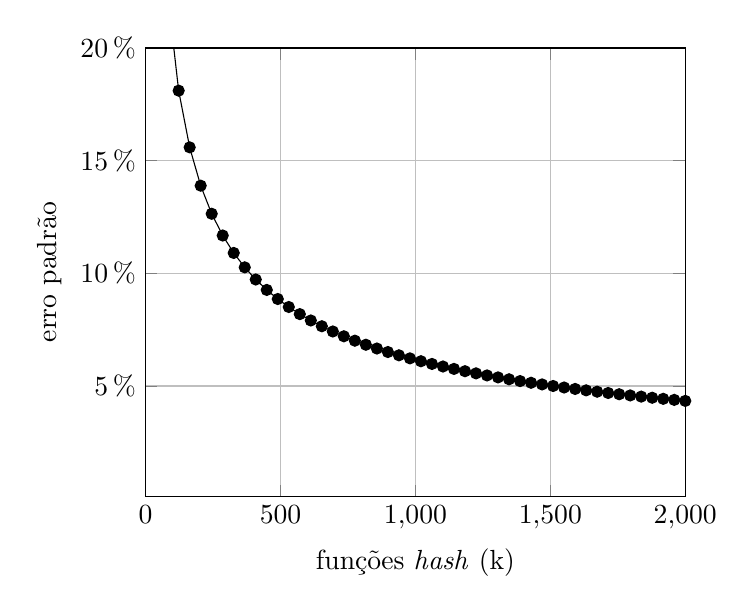
\begin{tikzpicture}[
        declare function = {
            p(\k,\c) = -(4 * sqrt(ln(2/\c)))/(sqrt(ln(2/\c))-sqrt(8*\k+ln(2/\c)));
        }
    ]
	\begin{axis}[
        grid=both,
        xlabel=funções \emph{hash} (k),
		ylabel=erro padrão,
		yticklabel=\pgfmathparse{100*\tick}\pgfmathprintnumber{\pgfmathresult}\,\%,
        ymin=0.001,
        ymax=0.20,
		xmin=0,
		xmax=2000]
	\addplot[mark=*,domain=0:2000,samples=50] {p(x, 0.317310508)};
	\end{axis}
\end{tikzpicture}}
\caption{Erro padrão por funções \emph{hash}}
\label{fig:min:prob}
\end{figure}

\subsection{Variante com apenas uma função \emph{hash}}

Muitas vezes, o custo de computar várias funções \emph{hash} pode ser muito alto na prática, especialmente para conjuntos com centenas de milhões de elementos.

Uma variante possível do \emph{MinHash} é utilizar apenas uma função \emph{hash} e manter os $k$ menores resultados em ordem ascendente de $h(x)$ para cada conjunto como assinatura (Algoritmo~\ref{alg:min:hashcompute2}). Denota-se por $h_{(k)}(S)$ o conjunto com $k$ menores hashes do conjunto $S$. 

\begin{algorithm}
\linespread{1}\selectfont
\caption{Computa a assinatura de um conjunto $S$}
\label{alg:min:hashcompute2}
\begin{algorithmic}[1]
\Function{Computar-Assinatura}{$S$}
    \State $H \gets \varnothing$
    \For{\text{each} $e \in S$}
        \State $H \gets H \cup h(e)$
        \If{$|H| > k$}
            \State $H \gets H - \{H_{\max}\}$
        \EndIf
    \EndFor
	\Return $H$
\EndFunction
\end{algorithmic}
\end{algorithm}

A similaridade entre os conjuntos será computada de uma forma diferente da variante com múltiplas funções \emph{hash}. Nesta, vale-se do princípio de que os $k$ menores elementos em $h_{(k)}(A) \cup h_{(k)}(B)$ são os mesmos que em $h_{(k)}(A \cup B)$. Assim, seja $Y = h_{(k)}(A \cup B) \cap h_{(k)}(A) \cap h_{(k)}(B)$.  $Y$ equivale aos membros de $h_{(k)}(A \cup B)$ que também estão em $ h_{(k)}(A \cap B)$. Pode-se, então, definir $|Y|/k$ como um estimador não-enviesado de $J(A, B)$ (Algoritmo~\ref{alg:min:hashcompare2}).

\begin{algorithm}
\linespread{1}\selectfont
\caption{Estimador de $J(A. B)$, sendo $H_1$ e $H_2$ as assinaturas, respectivamente, de $A$ e $B$}
\label{alg:min:hashcompare2}
\begin{algorithmic}[1]
\Function{Comparar-Assinaturas}{$H_1, H_2$}
    \State $H_x \gets k \text{ menores elementos de } H_1 \cup H_2 \ $
    \State $H_y \gets H_x \cap H_1 \cap H_2 $
	\Return $|H_y|/k$
\EndFunction
\end{algorithmic}
\end{algorithm}

Apesar da diferença prática, a ideia é similar à da variante com múltiplas funções \emph{hash}. Entretanto, nesta variante é preciso considerar que, em vez de obter apenas o primeiro elemento de cada permutação da matriz característica, obtém-se $k$ elementos. Mesmo assim, também é possível usar o limite de Chernoff para estimar o erro, pois o mesmo resultado para amostragem com substituição pode ser usado para amostragem sem substituição, como mostra Hoeffdin. \cite{hoeffding1963probability,bardenet2015concentration}.

\subsection{Detecção de quase-duplicatas}\label{sec:min:duplicate}

A motivação inicial que levou à criação do algoritmo \emph{MinHash} era encontrar quase-duplicatas em uma coleção de 30 milhões de documentos indexados pelo motor de busca Alta Vista em 1997 \cite{broder1997resemblance}. Percebe-se que apenas considerando a técnica \emph{hash}ing, a solução ainda é bastante impraticável, pois uma busca par-a-par no conjunto de dados requer $\binom{30,000,000}{2}$ -- ou aprox. 450 trilhões -- operações. Mesmo sendo capaz de executar cada comparação em 1 microsegundo, ainda levaria mais de uma década para processar a coleção inteira.

É importante notar, entretanto, que se o objetivo é encontrar grupos de similaridade, não é necessário computar o índice para todos os pares de conjuntos. É suficiente focar nos pares que possuem maior probabilidade de serem similares.

É possível utilizar a teoria \emph{hash}es sensíveis a localidade para diminuir a quantidade de pares a serem verificados. Uma técnica aplicável neste cenário é dividir as funções \emph{hash} em bandas e separar as assinaturas em baldes baseados no valor da assinatura em cada banda isoladamente. Assinaturas similares terão uma tendência maior de serem colocadas no mesmo balde (i.e. terem valores idênticos de assinatura naquela banda), com uma probabilidade definida.

Para entender a técnica, considere múltiplos conjuntos e a matriz formada por suas assinaturas \emph{MinHash}, utilizando a variante com múltiplas funções \emph{hash}. Cada coluna representa um conjunto e cada linha representa uma função \emph{hash}. O objetivo é separar as linhas em bandas e, para cada banda, verificar os grupos de assinaturas formados como candidatos a duplicatas. 

Por exemplo, na Figura~\ref{fig:minhash_signaturematrix} ilustra-se uma matriz de assinatura representando 5 conjuntos e 8 funções \emph{hash}, divididas em 4 bandas com 2 linhas cada.

\begin{figure}[!htbp]
\centering
\begin{tabular}{ c | c || c | c | c | c | c }
 banda & hash & $S_1$ & $S_2$ & $S_3$ & $S_4$ & $S_5$ \\
\hline
  \multirow{2}{*}{1} & $h_1$ & 6   & 1   & 7   & 6  & 2   \\
                     & $h_2$ & 1   & 3   & 7   & 1  & 3   \\
\hline
  \multirow{2}{*}{2} & $h_3$ & 8   & 3   & 8   & 5  & 3   \\
                     & $h_4$ & 0   & 9   & 4   & 1  & 9   \\
\hline
  \multirow{2}{*}{3} & $h_5$ & 2   & 0   & 6   & 2  & 0   \\
                       & $h_6$ & 0   & 0   & 3   & 1  & 0   \\
\hline
  \multirow{2}{*}{4} & $h_7$ & 5   & 1   & 1   & 5  & 1   \\
                     & $h_8$ & 4   & 4   & 9   & 4  & 4   \\
\end{tabular}
\caption{Matriz de assinaturas}
\label{fig:minhash_signaturematrix}
\end{figure}

No exemplo, a banda 2 revela um potencial par de quase-duplicatas, pois $S_2$ e $S_5$ possuem o mesmo valor para suas assinaturas naquela banda.

Considerando que deseja-se encontrar pares com similaridade acima de um certo limite, esta técnica está sujeita tanto a falsos positivos quantos falsos negativos. A probabilidade de um par de conjuntos $A$ e $B$, com $J(A, B) = s$, ser marcado como potencial duplicata, numa matriz com $b$ bandas com $r$ linhas por banda é exatamente a probabilidade dos dois conjuntos concordarem em todas as linhas de pelo menos uma banda, ou seja, $1 - (1 - s^r)^b$  \cite{rajaraman2012mining}.

Baseado nesta probabilidade, a Figura~\ref{fig:min:lshprob} mostra, em função da similaridade, a probabilidade de um par de documentos ser marcado como duplicado em uma matriz com 64 funções \emph{hash} e algumas escolhas de $b$ diferentes.

\begin{figure}[!htbp]
\centering
\scalebox{0.80}{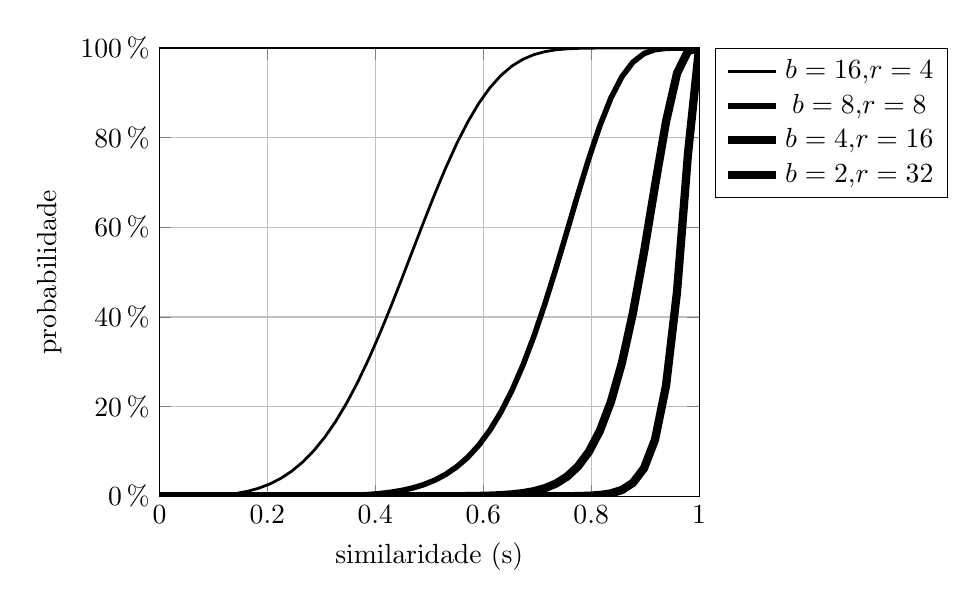
\begin{tikzpicture}[
        declare function = {
            p(\s,\b,\r) = 1 - (1 - \s^\r)^\b;
        }
    ]
	\begin{axis}[
        grid=both,
        xlabel=similaridade (s),
		ylabel=probabilidade,
		yticklabel=\pgfmathparse{100*\tick}\pgfmathprintnumber{\pgfmathresult}\,\%,
		ymin=0, ymax=1,
		xmin=0, xmax=1, 
		legend columns=1, 
	    legend style={legend pos=outer north east,}]
	\addplot[line width=1pt,domain=0:1,samples=50] {p(x, 16, 4)};
	\addplot[line width=2pt,domain=0:1,samples=50] {p(x, 8, 8)};
	\addplot[line width=3pt,domain=0:1,samples=50] {p(x, 4, 16)};
	\addplot[line width=3pt,domain=0:1,samples=50] {p(x, 2, 32)};
	\legend{$b=16 \text{, } r=4$, $b=8 \text{, } r=8$, $b=4 \text{, } r=16$, $b=2 \text{, } r=32$}
	\end{axis}
\end{tikzpicture}}
\caption{Probabilidade de ser escolhido como duplicata}
\label{fig:min:lshprob}
\end{figure}

Independente dos valores de $b$ e $r$ escolhidos, o gráfico sempre terá esta forma de "S". Entretanto, estes parâmetros definem com qual probabilidade um par de certa similaridade $s$ é considerado duplicado. Ainda assim, valores abaixo da similaridade definida podem ser considerados duplicados (falsos positivos) e valores acima podem ser ignorados (falsos negativos). 

A partir de $b$ e $r$ e uma probabilidade $p$ é possível derivar a partir de qual valor de similaridade se possui aquela probabilidade de ser escolhido, por inversão da função que fornece esta probabilidade:
\[
s = \left(1 - (1-p)^{1/b}\right)^{1/r}
\]

Por exemplo, $b=32$, $r=16$, temos 0.5\% de chance de encontrar um par de conjuntos com similaridade acima de $0.5683$, e 95\% de chance de encontrar pares com similaridade acima de $0.8891$. Ao manipular estes valores é possível dimensionar facilmente a tolerância a falsos positivos ou falsos negativos no algoritmo.

\subsection{\emph{SimHash}}

A partir do trabalho de Indyk e Motwani \cite{indyk1998approximate,gionis1999similarity}, começou-se a formalizar as bases teóricas das técnicas \emph{hash}ing sensível a localidade. De fato, \emph{MinHash} é apenas um tipo destes hashes. Muitos outros tipos foram estudados desde então. Uma dos mais bem sucedidos é o \emph{SimHash} \cite{charikar2002similarity}. Este algoritmo ganhou notoriedade nos últimos anos por compor um dos fatores usados pelo Google para priorizar a indexação de páginas na Internet \cite{manku2007detecting}.

Um hash sensível a localidade é definido por uma família de funções \emph{hash} $\mathcal{F}$, tal que para dois objetos $x, y \in U$, e uma certa função de similaridade $sim: U \times U \to {\rm I\!R}$, vale
\[
    \Pr_{h \in \mathcal{F}}[h(x) = h(y)] = sim(x, y)
\]

Em especial, para o \emph{MinHash}, o objetivo é estimar a similaridade entre conjuntos com um número grande de elementos, aproximando o índice de Jaccard, i.e. $sim(x, y) = J(x, y)$. Outras medidas podem ser utilizadas. 

No caso das assinaturas de Charikar -- ou \emph{SimHash} -- o objetivo é estimar a similaridade entre vetores em espaços de alta dimensão. Neste caso utiliza-se uma família de funções \emph{hash} baseadas no produto escalar entre vetores. No algoritmo, para comparar a similaridade em vetores em $\mathds{R}^d$, escolhe-se um vetor $\vec{r}$, de $d$ dimensões, onde cada coordenada é um valor escolhido aleatoriamente em uma distribuição gaussiana. Define-se a função como \[
    h_{\vec{r}}(\vec{u}) = \begin{cases} 
        1 & \text{se } \vec{r} \cdot \vec{u} \geq 0 \\
        0 & \text{se } \vec{r} \cdot \vec{u} < 0 \\
    \end{cases}
\]

Goemans e Williamson \cite{goemans1995improved} mostram que esta função respeita a definição suficiente para ser utilizada como um hash sensível a localidade, tal que, para vetores $\vec{u}$ e $\vec{v}$ 
\[
    \Pr[h_{\vec{r}}(\vec{u}) = h_{\vec{r}}(\vec{v})] = 1 - \frac{\theta(\vec{u}, \vec{v})}{\pi}\text{, }
\] 
onde $\theta(\vec{u}, \vec{v})$ é o menor ângulo formado por $\vec{u}$ e $\vec{v}$.

É possível utilizar esta família de funções para estimar a similaridade entre conjuntos. Cada elemento da união dos dois conjuntos seria associado a uma dimensão e cada conjunto representado como um vetor, tendo valor 1 nas dimensões respectivas aos elementos que contém. Por exemplo, sejam dois conjuntos $A$ e $B$:
\[
    A = \{a, d, e\} \text{ e } \\
    B = \{b, c, d, e\}
\]
uma possível definição dos vetores relativos a $A$ e $B$ seria:
\[
    v_A = (1, 0, 0, 1, 1) \text{ e } 
    v_B = (0, 1, 1, 1, 1)
\]

Como o menor ângulo formado por estes dois vetores é 1.15026rad, então a similaridade entre os dois, segundo esta métrica, é igual a aproximadamente 0.695913.

Para conjuntos, esta função \emph{hash} representa a seguinte métrica de similaridade:

\[
    \Pr[h_{\vec{r}}(\vec{u}_A) = h_{\vec{r}}(\vec{u}_B)] = 1 - \frac{\arccos \left( \frac{|A \cap B|}{\sqrt{|A| \cdot |B|}}\right)}{\pi}\text{.}
\]

Assim como no algoritmo \emph{MinHash}, porém mais claramente perceptível neste caso, uma função \emph{hash} perfeita iria requerer a representação do vetor $\vec{r}$ em $O(d)$ bits, o que em casos de alta dimensionalidade pode ser impraticável. Mas igualmente neste caso, mesmo famílias simples \emph{hash}es de Rabin são suficientes para uma boa aproximação \cite{charikar2002similarity}.

Na prática, o algoritmo consiste em computar $k$ bits \emph{hash} para cada elemento do conjunto, acumulando o sinal dos resultados em um vetor $V[1..k]$. O resultado é um outro vetor de $k$ bits, onde cada um assume o valor 0 se o respectivo valor no vetor acumulado for negativo e 1 se for não-negativo (Algoritmo~\ref{alg:min:simhashcompute}).

\begin{algorithm}
\linespread{1}\selectfont
\caption{Computa a assinatura \emph{SimHash} de um conjunto $S$}
\label{alg:min:simhashcompute}
\begin{algorithmic}[1]
\Function{Computar-Assinatura}{$S$}
    \For{$i \gets 1 \textrm{ to } k$}
        \State $v \gets 0$
        \For{\text{each} $e \in S$}
            \If{$h_i(e) \geq 0$}
                \State $v \gets v + 1$
            \Else
                \State $v \gets v - 1$
            \EndIf
	    \EndFor
        \State $H[i] \gets (v \geq 0)$
	\EndFor
	\Return $H$
\EndFunction
\end{algorithmic}
\end{algorithm}

A comparação entre assinaturas consiste em contar o número de bits iguais em duas assinaturas (Algoritmo~\ref{alg:min:simhashcompare}).

\begin{algorithm}
\linespread{1}\selectfont
\caption{Compara assinaturas \emph{SimHash} de conjuntos}
\label{alg:min:simhashcompare}
\begin{algorithmic}[1]
\Function{Comparar-Assinaturas}{$H_1, H_2$}
    \State $y \gets 0$
    \For{$i \gets 1 \textrm{ to } k$}
        \If{$H_1[i] = H_2[i]$}
            \State $y \gets y + 1$
        \EndIf
	\EndFor
	\Return $y/k$
\EndFunction
\end{algorithmic}
\end{algorithm}

Henzinger \cite{henzinger2006finding} argumenta que \emph{SimHash} tem um desempenho melhor ao estimar quase-duplicatas em documentos na Internet, se comparado ao \emph{MinHash}. Em especial, \emph{SimHash} requer menos espaço para atingir mesma precisão que \emph{MinHash}. Por outro lado, Shrivastava e Li \cite{shrivastava2014defense} afirmam que \emph{MinHash} é mais adequado que \emph{SimHash} para coleções de documentos com muitas similaridades.

Manku et al. \cite{manku2007detecting} descrevem a aplicabilidade desta técnica para detecção de quase-duplicatas usando assinaturas de 64 bits num banco de dados de 8 bilhões de páginas. Também sugerem um algoritmo otimizado para encontrar todas as assinaturas que diferem de uma assinatura específica em no máximo $k$ bits, onde $k$ é um inteiro pequeno.

\subsection{Aplicações}

O algoritmo \emph{MinHash} e outros mecanismos \emph{hash} sensíveis a localidade, têm enorme aplicação prática, especialmente como forma de oferecer uma função de similaridade e algoritmos de clusterização para os mais variados fins. Nesta seção listaremos alguns exemplos de aplicações comuns nesta área.

\begin{description}

\item[Sites de busca:]

Em seu trabalho seminal sobre \emph{MinHash}, Broder \cite{broder1997resemblance} já citava uma aplicação prática na indexação de páginas web pelo motor do Alta Vista, numa análise investigativa a fim de determinar quase-duplicatas em um índice de 30 milhões de documentos.

Manku et al. \cite{manku2007detecting} descrevem como usam, no Google, outra variante \emph{hash} sensível a localidade chamada \emph{SimHash}, baseada em distância entre vetores. No artigo, os autores introduzem uma técnica para determinar, a partir de coleção de 8 bilhões de páginas com assinaturas \emph{SimHash} de 64 bits pré-calculadas, se uma nova página encontrada pelo indexador possui uma duplicata já indexada.

\item[Bancos de dados de imagens:]

Embora hashing sensível a localidade seja mais comumente usado para comparação de documentos textuais, também é possível adaptá-lo para comparar a semelhança entre imagens. Neste caso, várias caracteristicas da imagem podem ser usadas como meio de comparação, desde histogramas de cores, parâmetros de iluminação, até os pixels individuais.

Ioffe \cite{ioffe2010improved} cita um caso de uso para uma variante do algoritmo \emph{MinHash}, modificada para permitir conjuntos ponderados, de modo a aproximar a distância $\ell_1$ entre vetores. No artigo, o objetivo principal é apresentar o uso da técnica, no Google, para busca aproximada por imagens num banco de dados. As imagens são representadas por vetores de features, como histogramas de cores e metadados. 

Lee et al. \cite{lee2010partition} também descrevem um método para busca parcial de imagens usando \emph{MinHash}. Neste caso, o objetivo é agrupar imagens que provavelmente contém um mesmo objeto, mesmo que as imagens não sejam inteiramente compostas por ele.

Numa aplicação mais clássica, Wang et al. \cite{wang2013duplicate} expõem os resultados alcançados pela divisão Microsoft Research em uma busca por duplicatas em uma coleção de mais de 2 bilhões de imagens da Internet. Utilizando uma variante em dois passos do \emph{MinHash}, eles foram capazes de encontrar mais de 500 milhões de imagens duplicadas em 13 horas de processamento em um cluster de 2.000 núcleos.

\item[Sistemas de recomendação:]

A capacidade de verificar a semelhança entre conjuntos ou vetores abre portas para aplicação de \emph{MinHash} em algoritmos de clusterização baseados em similaridade.

O serviço de notícias Google News utiliza \emph{MinHash} para seu mecanismo de recomendação de artigos para os usuários \cite{das2007google}. A recomendação é calculada em tempo real com latência abaixo de um segundo. Para tanto, os autores descrevem como utilizam aprendizado de máquina, aplicando \emph{MinHash} como função de similaridade. Todo o processamento é realizado no modelo MapReduce, para permitir a criação de um mecanismo de recomendação de notícias com alta escalabilidade.

Além disso, Rodrigues \cite{rodrigues2013recomendaccao} sugere a utilização de \emph{MinHash} para clusterização de espectadores em serviços de TV, baseados nas opções pregressas.

\item[Similaridade em Redes Sociais:]

A detecção de comunidades orgânicas em redes sociais é um problema cada vez mais comum atualmente. O problema pode ser modelado como um caso especial de sistema de recomendação, onde o objetivo é clusterizar nós comuns num grafo por um conjunto de características. 

Macropol e Singh \cite{macropol2010scalable} introduzem em 2010 o algoritmo \emph{Top Graph Clusters} (\emph{TopGC}), utilizando hashes sensíveis a localidade -- especialmente \emph{MinHash} -- para detecção, em tempo linear, de subgrafos altamente conectados. O algoritmo propõe utilizar, como métrica de afinidade entre os nós, a semelhança entre suas vizinhanças.

Teixeira et al. \cite{teixeira2012min} descrevem como utilizar \emph{MinHash} como função de similaridade, com o objetivo de computar a semelhança entre grafos utilizando poucos recursos.


\end{description}

\subsection{Resultados experimentais}\label{sec:min:experiments}

Para melhor observar as previsões teóricas sobre o algoritmo \emph{MinHash}, conduzimos uma série de experimentos para verificar empiricamente as probabilidades descritas na teoria. Testamos tanto a variante com múltiplas funções \emph{hash} quanto com apenas uma função. Testamos também a técnica de clusterização de pares duplicados descrita na Seção~\ref{sec:min:duplicate}.

Para todos os testes, foi utilizado um conjunto de dados misto, composto por todas as obras de Shakespeare (42 obras, 964410 palavras, 23704 distintas). Para cada obra, consta no conjunto de dados o conjunto de palavras distintas da obra, bem como uma cópia deste conjunto com uma certa porcentagem aleatória de palavras substituídas por strings aleatórias (84 conjuntos de palavras foram utilizados no total).

Em todos os casos, a família de funções \emph{hash} utilizada foi MurmurHash 3 \cite{appleby2012murmur}, de 32 bits. Várias funções foram geradas, usando sementes diferentes.

A métrica de similaridade utilizada no teste foi o índice de Jaccard entre os conjuntos simples de palavras de cada texto. Este índice foi calculado de forma determinística para os $\binom{42 \times 2}{2} = 3486$ pares de documentos. A distribuição de similaridades entre os pares pode ser vista no histograma da Figura~\ref{fig:minhash_dist}.

\begin{figure}[!htbp]
\centering
\scalebox{0.80}{\begin{tikzpicture}
	\begin{semilogyaxis}[
	    ybar,
	    xmin=0, xmax=1
    ]

    \addplot +[
        fill=gray!25,
        draw=gray!100,
        hist={
            bins=10,
            data min=0,
            data max=1
        }   
    ] table [y index=0] {files/minhash_dist.txt};

	\end{semilogyaxis}
\end{tikzpicture}}
\caption{Distribuição de similaridades entre pares de documentos}
\label{fig:minhash_dist}
\end{figure}


Para os dois testes, variou-se $k$ (o número de funções \emph{hash}) entre 25 e 1000. Mediu-se então, para cada par, o quanto o estimador da similaridade desviava do valor real (calculado deterministicamente). Para estes valores foram computados a média, e o desvio padrão. A Figura \ref{fig:min:result} mostra os resultados obtidos para as variantes de múltiplas funções e apenas uma função \emph{hash}, respectivamente. Na figura é possível comparar com o intervalo esperado pela teoria apresentada, com 95\% de certeza.

\begin{figure}[!htbp]
\centering
\scalebox{0.80}{\begin{tikzpicture}[
        declare function = {
            p(\k,\c) = -(4 * sqrt(ln(2/\c)))/(sqrt(ln(2/\c))-sqrt(8*\k+ln(2/\c)));
        }
    ]
	\begin{axis}[
	    title=Múltiplas funções \emph{hash},
	    scaled ticks=false, 
        grid=both,
        ylabel={erro},
        xlabel=tamanho da assinatura ($k$),
		yticklabel=\pgfmathparse{100*\tick}\pgfmathprintnumber{\pgfmathresult}\,\%,
		ymin=0,ymax=0.3,ystep=0.01,
		xmin=0, xmax=1000, 
		legend columns=1, 
	    legend style={legend pos=outer north east,}
    ]

    \addplot[line width=15pt,domain=0:1,samples=30,color={rgb:black,1;white,1},opacity=0.4]{2};

    \addplot[name path=line3, line width=0pt,domain=1:1000,samples=40,opacity=0.0,forget plot]{p(x, 0.31731)*sqrt(2)/sqrt(pi)};
    \addplot[name path=line4, line width=15pt,domain=1:1000,samples=30,opacity=0.0, forget plot]{0};

	\addplot[fill={rgb:black,1;white,1},fill opacity=0.40,forget plot] fill between[ of = line3 and line4];

	\addplot[line width=1pt, mark=*,black,smooth, mark options={scale=0.75}] table[x=k,y=mean] {files/minhash_shakespeare.txt};
	\addplot[dashed, line width=1pt, mark=none,black,smooth, mark options={scale=0.75}] table[x=k,y=stdev] {files/minhash_shakespeare.txt};
	%\addplot[dotted, line width=1pt, mark=none,black,smooth] table[x=k,y=max] {files/minhash_shakespeare.txt};
	%\legend{esperado,shakespeare, $\pm 1 \sigma$, min/max };


	\end{axis}
\end{tikzpicture} \begin{tikzpicture}[
        declare function = {
            p(\k,\c) = -(4 * sqrt(ln(2/\c)))/(sqrt(ln(2/\c))-sqrt(8*\k+ln(2/\c)));
        }
    ]
	\begin{axis}[
	    title=Única função \emph{hash},
	    scaled ticks=false, 
        grid=both,
        xlabel=tamanho da assinatura ($k$),
		yticklabel={\ },
		ymin=0,ymax=0.3,ystep=0.01,
		xmin=0, xmax=1000, 
		legend columns=1, 
	    %legend style={legend pos=outer north east,}
    ]

    \addplot[line width=15pt,domain=0:1,samples=30,color={rgb:black,1;white,1},opacity=0.4]{2};

    \addplot[name path=line3, line width=0pt,domain=1:1000,samples=40,opacity=0.0,forget plot]{p(\x, 0.31731)*sqrt(2)/sqrt(pi)};
    \addplot[name path=line4, line width=15pt,domain=1:1000,samples=30,opacity=0.0, forget plot]{0};
	\addplot[fill={rgb:black,1;white,1},fill opacity=0.40,forget plot] fill between[ of = line3 and line4];

	\addplot[line width=1pt, mark=*,black,smooth, mark options={scale=0.75}] table[x=k,y=mean] {files/minhash_shakespeare2.txt};
	\addplot[dashed, line width=1pt, mark=none,black,smooth, mark options={scale=0.75}] table[x=k,y=stdev] {files/minhash_shakespeare2.txt};
	%\addplot[dotted, line width=1pt, mark=none,black,smooth] table[x=k,y=max] {files/minhash_shakespeare2.txt};
	\legend{esperado, média, $+1\sigma$, máximo };

	\end{axis}
\end{tikzpicture}}
\caption{Erro observado por funções \emph{hash}}
\label{fig:min:result}
\end{figure}

Também foi realizado o teste de clusterização dos pares de documentos utilizando a técnica descrita na Seção~\ref{sec:min:duplicate}. 

Inicialmente calculou-se, para cada documento, assinaturas \emph{MinHash} com 512 funções \emph{hash}. Utilizou-se então a técnica de clusterização utilizando todas as possíveis combinações de número de bandas ($b$) e linhas por banda ($r$). 

\begin{figure}[!htbp]
\centering
\scalebox{0.80}{\begin{tikzpicture}[
        declare function = {
            p(\b,\r,\p) = (1 - (1-\p)^(1/\b))^(1/\r);
        }
    ]
	\begin{axis}[
	    xmode=log,
	    log basis x=2,
	    scaled ticks=false, 
        grid=both,
        xlabel=número de bandas ($b$),
		ylabel=similaridade ($s$),
		ymin=0,ymax=1,
		xmin=8,xmax=512, 
		legend columns=1, 
	    legend style={legend pos=outer north east,},
	    legend cell align=left
    ]

    \addplot[line width=15pt,domain=8:9,samples=2,color={rgb:black,1;white,1},opacity=0.4]{2};
    \addplot[line width=15pt,domain=8:9,samples=2,color={rgb:black,1;white,1},opacity=0.7]{2};


    \addplot[name path=line3, line width=0pt,domain=8:512,samples=40,opacity=0.0,forget plot] table[x=b,y=max] {files/minhash_calculated.txt};
    \addplot[name path=line4, line width=0pt,domain=8:512,samples=40,opacity=0.0,forget plot] table[x=b,y=min] {files/minhash_calculated.txt};
    \addplot[name path=line5, line width=0pt,domain=8:512,samples=40,opacity=0.0,forget plot]{1};
	\addplot[fill={rgb:black,1;white,1},fill opacity=0.40,forget plot] fill between[ of = line3 and line4];
	\addplot[fill={rgb:black,1;white,1},fill opacity=0.70,forget plot] fill between[ of = line5 and line3];

	\addplot[only marks, mark=*,opacity=1,black,mark options={scale=0.75}] table[x=b,y=v] {files/minhash_detect.txt};
    
    \legend{$0.5\%<P<99.5\%$,$P\geq99.5\%$, pares encontrados };


	\end{axis}
\end{tikzpicture}}
\caption{Pares detectados para cada configuração de bandas.}
\label{fig:min:detect}
\end{figure}

As similaridades dos pares encontrados com cada configuração, bem como a comparação com o valor predito pela teoria podem ser vistos na Figura~\ref{fig:min:detect}. Configurações que resultaram em nenhum par encontrado são omitidas por brevidade.

É importante notar no resultado não só valores abaixo da probabilidade de corte (falsos positivos), como muitos valores de similaridade altos omitidos numa certa configuração de bandas, mas que aparecem na próxima (falsos negativos).